\documentclass{beamer}

\usepackage{beamerthemesplit}
\usepackage{amsmath}
\usepackage{amsfonts}
\usepackage{amssymb}
\usepackage{qtree}
\usepackage{cancel}

\newcommand{\df}{\mu} %probability density function
\newcommand{\dfo}{\nu} %other probability density function
\newcommand{\fv}{x} %fuzzy variable
\newcommand{\an} {\alpha} %angle variable
\newcommand{\ano}{\beta} %other angle variable
\newcommand{\newtv}{\varphi}
\newcommand{\PZ}{\mathcal{P}(\mathcal{Z})}
\newcommand{\CFPl}{fuzzy-probabilistic} %classical fuzzy-probabilistic connector
\newcommand{\CFP}{FP} %classical fuzzy-probabilistic connector
\newcommand{\XFPl}{distributional fuzzy} %extended fuzzy-probabilistic connector
\newcommand{\XFP}{DF} %extended fuzzy-probabilistic connector

\newcommand{\MODELS}{\vdash}

%RCC relationships
\newcommand{\PR}{{\tt P}}
\newcommand{\PRl}{{\tt PartOf}}
\newcommand{\PRFl}{{\tt PartOf}^{\it fuz}}
\newcommand{\CR}{{\tt C}}
\newcommand{\CRl}{{\tt Connected}}
\newcommand{\DCR}{{\tt DC}}
\newcommand{\DCRl}{{\tt Disconnected}}
\newcommand{\ECR}{{\tt EC}}
\newcommand{\ECRl}{{\tt ExternallyConnected}}
\newcommand{\EQR}{{\tt EQ}}
\newcommand{\EQRl}{{\tt Equal}}
\newcommand{\OR}{{\tt O}}
\newcommand{\ORl}{{\tt Overlap}}
\newcommand{\IR}{{\tt I}}
\newcommand{\IRl}{{\tt Inside}}
\newcommand{\NR}{{\tt N}}
\newcommand{\NRl}{{\tt Near}}
\newcommand{\FR}{{\tt F}}
\newcommand{\FRl}{{\tt Far}}
\newcommand{\BIGR}{{\tt B}}
\newcommand{\BIGRl}{{\tt Big}}
\newcommand{\LONGR}{{\tt L}}
\newcommand{\LONGRl}{{\tt Long}}

%universe
\newcommand{\Un}{\mathcal{U}}

%Allen relationships
\newcommand{\DR}{{\tt D}}
\newcommand{\DRl}{{\tt During}}
\newcommand{\BR}{{\tt B}}
\newcommand{\BRl}{{\tt Before}}
\newcommand{\MR}{{\tt M}}
\newcommand{\MRl}{{\tt Meet}}
\newcommand{\AR}{{\tt A}}
\newcommand{\ARl}{{\tt After}}

%PLN
%Various links
\newcommand{\IMPL}{{\tt ImplicationLink}} 
\newcommand{\IMPLHOF}{{\tt ImplicationLink\_HOF}} 
\newcommand{\AND}{{\tt ANDLink}}
\newcommand{\FORALL}{{\tt ForAllLink}}
\newcommand{\LIST}{{\tt ListLink}}
\newcommand{\EXOUT}{{\tt ExOutLink}}
\newcommand{\EVAL}{{\tt EvaluationLink}}
%variables
\newcommand{\VX}{{\tt \$X}}
\newcommand{\VY}{{\tt \$Y}}
\newcommand{\VZ}{{\tt \$Z}}
\newcommand{\VIA}{{\tt \$I_1}}
\newcommand{\VIB}{{\tt \$I_2}}
\newcommand{\VIC}{{\tt \$I_3}}
%truth value
\newcommand{\TV}{{\tt tv}}
\newcommand{\TVA}{{\tt tv_1}}
\newcommand{\TVB}{{\tt tv_2}}
\newcommand{\TVC}{{\tt tv_3}}
\newcommand{\TVD}{{\tt tv_4}}
\newcommand{\TVE}{{\tt tv_5}}
\newcommand{\TVF}{{\tt tv_6}}
\newcommand{\TVG}{{\tt tv_7}}
\newcommand{\TVH}{{\tt tv_8}}
\newcommand{\TVI}{{\tt tv_9}}
\newcommand{\BTV}{\langle \TV \rangle}
\newcommand{\BTVA}{\langle \TVA \rangle} 
\newcommand{\BTVB}{\langle \TVB \rangle} 
\newcommand{\BTVC}{\langle \TVC \rangle} 
\newcommand{\BTVD}{\langle \TVD \rangle} 
\newcommand{\BTVE}{\langle \TVE \rangle}
\newcommand{\BTVF}{\langle \TVF \rangle} 
\newcommand{\BTVG}{\langle \TVG \rangle} 
\newcommand{\BTVH}{\langle \TVH \rangle} 
\newcommand{\BTVI}{\langle \TVI \rangle} 
%Tabulation space
\newcommand{\SP}{\qquad}

\mode<presentation>
{
  \usetheme{Warsaw}
  % or ...

  %\setbeamercovered{transparent}
  % or whatever (possibly just delete it)
}


\usepackage[english]{babel}
% or whatever

\usepackage[latin1]{inputenc}
% or whatever

\usepackage{times}
\usepackage[T1]{fontenc}


%%%%%%%%% NEW COMMANDS %%%%%%%%%
\newcommand{\score}{{\it score}}
\newcommand{\fitness}{{\it fitness}}
\newcommand{\sizepenalty}{{\it sizePenalty}}
\newcommand{\pset}[1]{\Theta_i(#1)}
\newcommand{\argmax}[1]{\underset{#1}{\operatorname{argmax}}\ }
\newcommand{\argmin}[1]{\underset{#1}{\operatorname{argmin}}\ }
\newcommand{\stos}{f_i}
\newcommand{\stof}{g_i}


\title{Uncertain Spatiotemporal Logic for AGI}
\subtitle{PLN and the OpenCog Framework}
\author{Nil Geisweiller \& Ben Goertzel}
\institute[IDSIA] % (optional, but mostly needed)
{
  Novamente LLC
}

\date[AGI-10] % (optional, should be abbreviation of conference name)
{AGI-10}

\begin{document}

\frame
{
  \maketitle
}

\frame
{
  \frametitle{Motivation: \alert{Spatiotemporal reasoning} within OpenCog}
  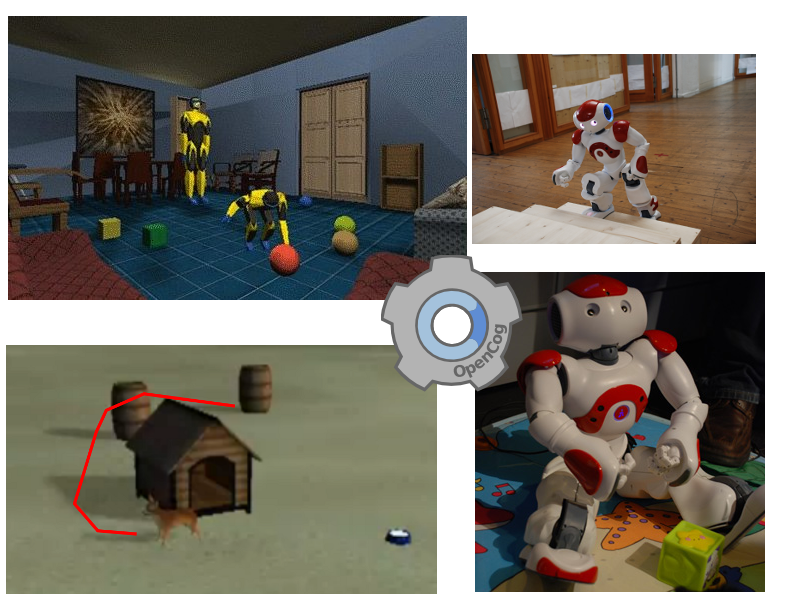
\includegraphics[scale=0.36]{opencog.png}
}

\frame
{
  \frametitle{Existing Spatiotemporal Calculi: \alert{Space}}
  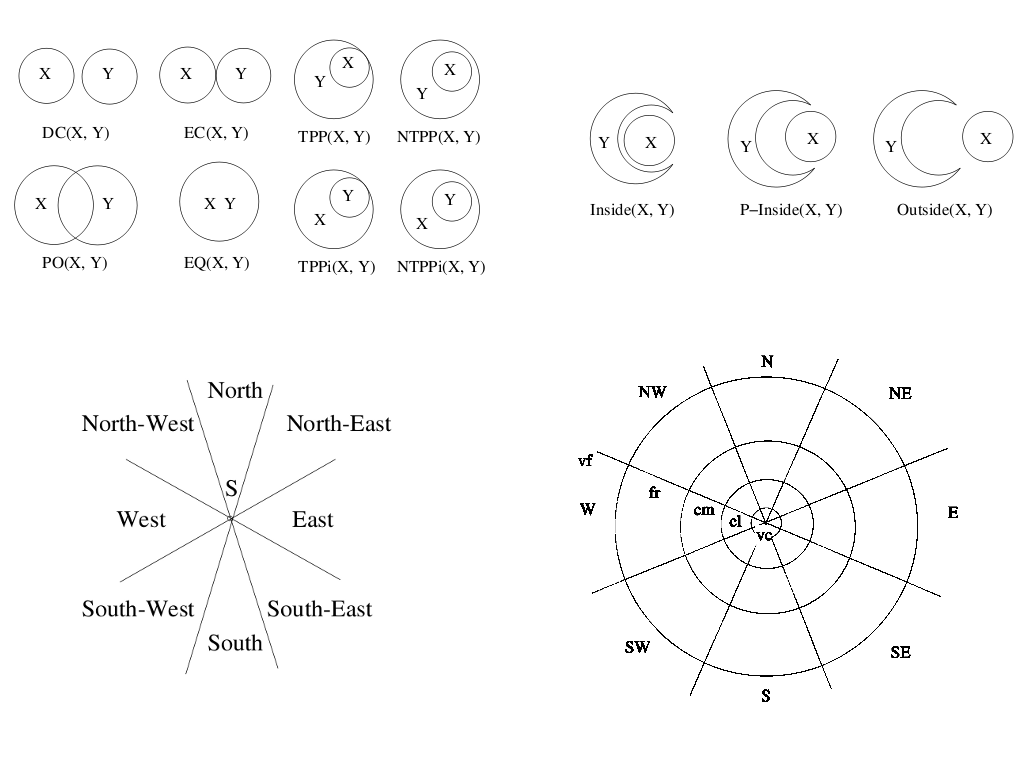
\includegraphics[scale=0.36]{space.png}
}

\frame
{
  \frametitle{Existing Spatiotemporal Calculi: \alert{Time}}
  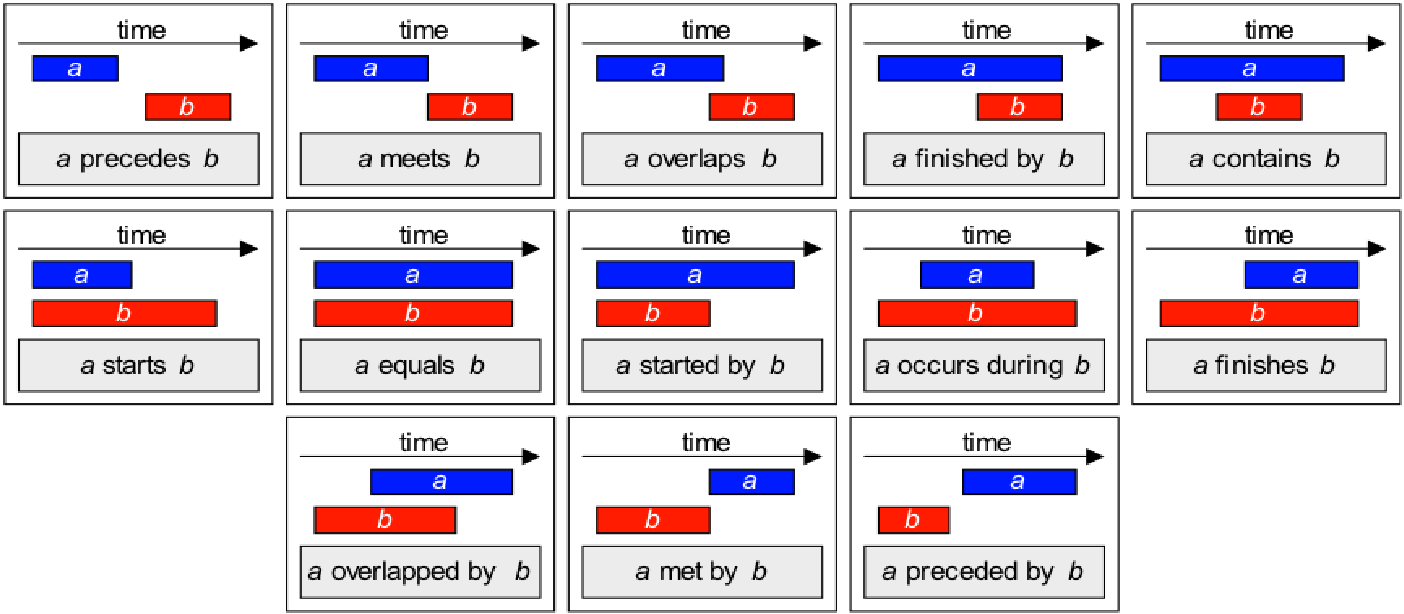
\includegraphics[scale=0.30]{Allen.png}
}

\frame
{
  \frametitle{Existing Spatiotemporal Calculi: \alert{Motion}}
  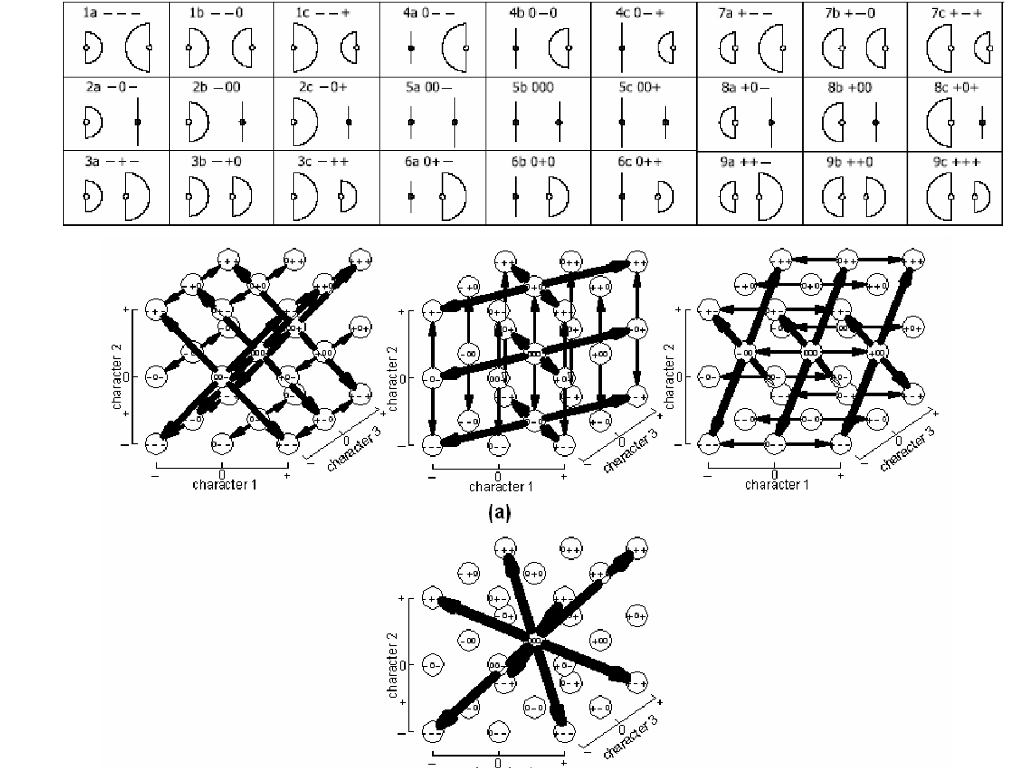
\includegraphics[scale=0.36]{motion.png}
}

\frame
{
  \frametitle{\alert{Uncertainty} in Spatiotemporal Calculi}

  \begin{itemize}
  \item<+-> There exist \alert{fuzzy} extensions, but too much uncertainties\\
    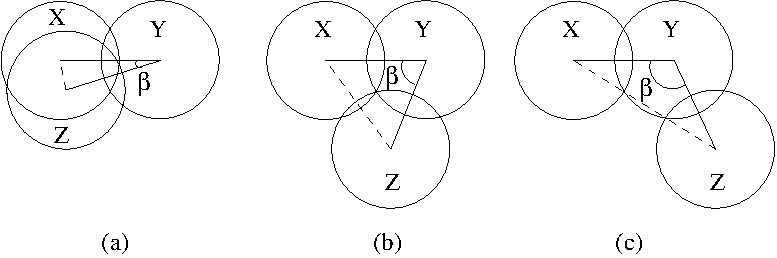
\includegraphics[scale=0.4]{circles3Conf.pdf} = Total uncertainty \alert{[0,1]}
  \item<+-> However with \alert{fuzzy-probabilistic} extension (similar to YKY's PZ-logic but with PLN TruthValue)
    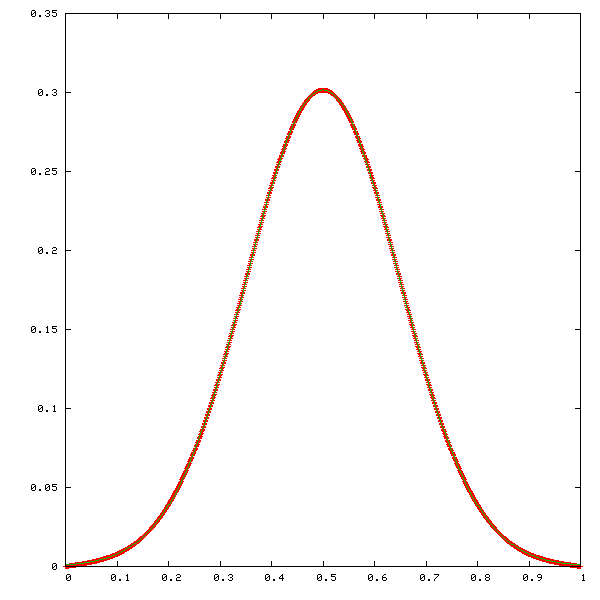
\includegraphics[scale=0.2]{gaussian_pulse_1d.png}
  \end{itemize}
}

\frame
{
  \frametitle{The math... in 10s}
  \begin{equation*}
    \label{eq:fuzzyprob}
    \begin{array}{c}
      \df_F =
      \underbrace{\displaystyle\int_0^1 \ldots \displaystyle\int_0^1}_n 
      F(\fv_1, \ldots, \fv_n) \df_1(\fv_1)\ldots\df_n(\fv_n)d\fv_1\ldots d\fv_n
    \end{array}
  \end{equation*}

  Example of PLN rule for $\PRl$ transitivity

  \begin{equation*}
    \begin{array}{|l|}
      \hline
      \FORALL\ \VX\ \VY\ \VZ\\
      \SP \IMPLHOF\\
      \SP\SP \AND\\
      \SP\SP\SP \PRl(\VX,\VY)\ \BTVA\\
      \SP\SP\SP \PRl(\VY,\VZ)\ \BTVB\\
      \SP\SP \AND\\
      \SP\SP\SP \TVC = \df_{F}(\TVA,\TVB)\\
      \SP\SP\SP \PRl(\VX,\VZ)\ \BTVC\\
      \hline
    \end{array}
  \end{equation*}
}

\frame
{
  \frametitle{Example: fetching the toy inside the upper cupboard}
  \begin{beamerboxesrounded}{Axioms}
      {\tiny
        \begin{enumerate}
        \item The toy is near the bag and inside the cupboard. The pillow is near and below the cupboard\\
          $
          \begin{array}{l}
            \NRl({\tt toy}, {\tt bag})\ \BTVA\\
            \IRl({\tt toy}, {\tt cupboard})\ \BTVB\\
            {\tt Below}({\tt pillow}, {\tt cupboard})\ \BTVC\\
            \NRl({\tt pillow}, {\tt cupboard})\ \BTVD\\
          \end{array}
          $
        \item The toy is near the bad inside the cupboard, how much the
          toy is near the edge of the cupboard?
          $
          \begin{array}{l}
            \IMPLHOF\\
            \SP \AND\\
            \SP \SP \NRl({\tt toy}, {\tt bag})\ \BTVA\\
            \SP \SP \IRl({\tt toy}, {\tt cupboard})\ \BTVB\\
            \SP \AND\\
            \SP \SP \TVC = \df_{F_1}(\TVA, \TVB)\\
            \SP \SP \NRl({\tt toy}, {\tt cupboard\_edge})\ \BTVC
          \end{array}
          $
        \item If I climb on the pillow, then shortly after I'll be on the pillow\\
          $
          \begin{array}{l}
          {\tt PredictiveImplicationLink}\\
          \SP {\tt Climb\_on}({\tt pillow})\\
          \SP {\tt Over}({\tt self}, {\tt pillow})
          \end{array}
          $
        \item If I am on the pillow near the edge of the cupboard how
          near am I from the toy?
          $
          \begin{array}{l}
          \IMPLHOF\\
          \SP \AND\\
          \SP \SP {\tt Below}({\tt pillow}, {\tt cupboard})\ \BTVA\\
          \SP \SP {\tt Near}({\tt pillow}, {\tt cupboard})\ \BTVB\\
          \SP \SP {\tt Over}({\tt self}, {\tt pillow})\ \BTVC\\
          \SP \SP \NRl({\tt toy}, {\tt cupboard\_edge})\ \BTVD\\
          \SP \AND\\
          \SP \SP \TVE = \df_{F_2}(\TVA, \TVB, \TVC, \TVD)\\
          \SP \SP \NRl({\tt self}, {\tt toy})\ \BTVE\\
          \end{array}
          $          
        \end{enumerate}
      }
  \end{beamerboxesrounded}
}

\frame
{
  \frametitle{Example: fetching the toy inside the upper cupboard}
  \begin{beamerboxesrounded}{Target Theorem}
    {\tiny
      How near I am from the toy if I climb on the pillow\\
      $
      \begin{array}{l}
        {\tt PredictiveImplicationLink}\\
        \SP {\tt Climb\_on}({\tt pillow})\\
        \SP \NRl({\tt self}, {\tt toy})\ {\langle ? \rangle}\\
      \end{array}
      $
    }
  \end{beamerboxesrounded}
  \begin{beamerboxesrounded}{Inference}
    {\tiny
        \begin{enumerate}
        \item Axiom 2 with axiom 1\\
          $\NRl({\tt toy}, {\tt cupboard\_edge})\ \BTVF$
        \item Step 1 with axiom 1 and 3\\
          $
          \begin{array}{l}
            {\tt PredictiveImplicationLink}\\
            \SP {\tt Climb\_on}({\tt pillow})\\
            \SP \AND\\
            \SP \SP {\tt Below}({\tt pillow}, {\tt cupboard})\ \BTVC\\
            \SP \SP {\tt Near}({\tt pillow}, {\tt cupboard})\ \BTVD\\
            \SP \SP {\tt Over}({\tt self}, {\tt pillow})\ \BTVG\\
            \SP \SP \NRl({\tt toy}, {\tt cupboard\_edge})\ \BTVF\\
          \end{array}
          $
        \item Step 2 with axiom 4, target theorem: How near I am from
          the toy if I climb on the pillow\\
          $
          \begin{array}{l}
            {\tt PredictiveImplicationLink}\\
            \SP {\tt Climb\_on}({\tt pillow})\\
            \SP \NRl({\tt self}, {\tt toy})\ \BTVI\\
          \end{array}
          $
        \end{enumerate}
    }
  \end{beamerboxesrounded}
}

\frame
{
  \frametitle{Conclusion}
  \begin{itemize}
  \item Fuzzy-probabilistic seems \alert{more accurate}
  \item No need to be overkill either, \alert{adjustable precision}
  \item Perfectly \alert{adequate for OpenCog}'s reasoning engine PLN
    \begin{itemize}
    \item Uncertain Reasoning
    \item Learning or improving rules
    \end{itemize}
  \end{itemize}
  Still need to implement and experiment...
}

\end{document}
